% ═══════════════════════════════════════════════════════════════════════════
%  QASecClaw: LLM-Augmented Multi-Agent Framework for False Positive
%  Reduction in Static Application Security Testing
%  Pre-release Draft — Author(s) TBD
% ═══════════════════════════════════════════════════════════════════════════
\documentclass[conference]{IEEEtran}

\usepackage[utf8]{inputenc}
\usepackage[T1]{fontenc}
\usepackage{amsmath,amssymb}
\usepackage{graphicx}
\usepackage{booktabs}
\usepackage{hyperref}
\usepackage{xcolor}
\usepackage{balance}
\usepackage{multirow}
\usepackage{array}
\usepackage{url}
\usepackage{cite}
\usepackage{subcaption}
\usepackage{tabularx}

\hypersetup{
  colorlinks=true,
  linkcolor=blue!70!black,
  citecolor=blue!70!black,
  urlcolor=blue!60!black
}

\graphicspath{{../figures/}}

\begin{document}

\title{QASecClaw: LLM-Augmented Multi-Agent Framework for\\ False Positive Reduction in Static Application Security Testing}

\author{
  \textit{Author(s) — To Be Determined}\\
  \textit{Pre-release Draft}
}

\maketitle

% ═══════════════════════════════════════════════════════════════════════════
%  ABSTRACT
% ═══════════════════════════════════════════════════════════════════════════
\begin{abstract}
Static Application Security Testing (SAST) tools are critical components of modern secure software development pipelines, yet they produce prohibitively high false positive rates that erode developer trust and impose significant triage overhead. We present \textbf{QASecClaw}, a multi-agent orchestration framework that augments conventional SAST engines with Large Language Model (LLM)-driven contextual code review to substantially reduce false positives while preserving high recall. QASecClaw employs a pipeline of specialized agents — including a Test Planning Agent, a Security Validation Agent backed by Semgrep, and a novel SAST Filter Agent powered by an LLM — coordinated by a Mission Orchestrator that manages the analysis lifecycle. We evaluate QASecClaw on the complete \textbf{OWASP Benchmark v1.2}, a widely recognized synthetic vulnerability suite comprising 2,740 Java test cases across 11 CWE categories with built-in ground-truth labels. Our experimental results demonstrate that QASecClaw achieves an F1-score of \textbf{0.9093} compared to the standalone Semgrep baseline of \textbf{0.7839}, driven by an 88.6\% reduction in false positives (from 560 to 64) with only a 3.1\% decrease in recall. Per-CWE analysis reveals consistent improvements across injection, cryptographic, and access control vulnerability classes, with notably strong performance on SQL Injection (F1: 0.9405), XSS (F1: 0.8958), and Weak Cryptography (F1: 0.9961). These results validate the viability of LLM-augmented multi-agent architectures as a practical and scalable approach to improving the signal-to-noise ratio of SAST output.
\end{abstract}

\begin{IEEEkeywords}
Static Application Security Testing, False Positive Reduction, Large Language Models, Multi-Agent Systems, OWASP Benchmark, Software Security
\end{IEEEkeywords}

% ═══════════════════════════════════════════════════════════════════════════
%  I. INTRODUCTION
% ═══════════════════════════════════════════════════════════════════════════
\section{Introduction}
\label{sec:introduction}

Security vulnerabilities in software applications remain a pervasive and costly problem. Organizations increasingly rely on Static Application Security Testing (SAST) tools to identify potential vulnerabilities early in the development lifecycle, before deployment~\cite{chess2004static}. However, the practical adoption of SAST tools is severely constrained by their characteristically high false positive rates. Studies have shown that SAST tools can produce false positive rates exceeding 50\%, meaning that more than half of all reported findings are non-exploitable or benign code patterns~\cite{johnson2013don, sadowski2015tricorder}. This alert fatigue leads to wasted developer effort in triaging non-issues and, paradoxically, causes real vulnerabilities to be overlooked as teams begin to distrust and ignore scanner output.

Recent advances in Large Language Models (LLMs) have demonstrated remarkable capabilities in code understanding, generation, and analysis~\cite{chen2021evaluating, feng2020codebert}. These models can reason about data flows, identify sanitization patterns, and understand the semantic context of code in ways that rule-based SAST engines cannot. Simultaneously, the multi-agent systems paradigm~\cite{wooldridge2009introduction} has emerged as a powerful architectural pattern for decomposing complex tasks into specialized, cooperating agents.

In this paper, we present \textbf{QASecClaw}, a multi-agent framework that combines traditional SAST scanning with LLM-driven contextual code review to systematically reduce false positives while maintaining high vulnerability detection rates. Our key contributions are:

\begin{enumerate}
    \item \textbf{A multi-agent orchestration architecture} that decomposes the security assessment pipeline into specialized agents coordinated by a central Mission Orchestrator, enabling modular and extensible security analysis.
    \item \textbf{An LLM-augmented SAST Filter Agent} that performs deep code review on SAST findings, analyzing data flows and execution sinks to classify findings as true positives or false positives based on semantic understanding of vulnerability patterns.
    \item \textbf{A comprehensive empirical evaluation} on the complete OWASP Benchmark v1.2 (2,740 test cases, 11 CWE categories), demonstrating an F1-score improvement from 0.7839 to 0.9093 over standalone SAST, driven by an 88.6\% reduction in false positives.
\end{enumerate}

% ═══════════════════════════════════════════════════════════════════════════
%  II. RELATED WORK
% ═══════════════════════════════════════════════════════════════════════════
\section{Related Work}
\label{sec:related}

\subsection{Static Application Security Testing}
SAST tools such as Semgrep~\cite{semgrep2023}, SonarQube~\cite{sonarqube2023}, and Fortify~\cite{chess2004static} analyze source code without execution to identify potential vulnerabilities. These tools rely on pattern matching, taint analysis, and data flow tracking against known vulnerability signatures. While effective at achieving high recall, they suffer from substantial false positive rates because they lack execution context and often cannot reason about complex sanitization logic~\cite{johnson2013don}.

\subsection{False Positive Reduction Techniques}
Prior work on reducing SAST false positives has explored several directions. Hybrid analysis approaches combine static and dynamic techniques to validate findings~\cite{lam2017combining}. Machine learning classifiers have been trained to distinguish true from false positives based on code features~\cite{delaitre2015nist, flynn2018prioritizing}. More recently, deep learning models have been applied to vulnerability detection~\cite{li2021vulnerability, zhou2019devign}. However, these approaches often require substantial labeled training data and may not generalize across vulnerability types.

\subsection{LLMs for Code Security}
The application of LLMs to security analysis is an emerging research direction. Studies have explored using LLMs for vulnerability detection~\cite{thapa2022transformer}, automated patch generation~\cite{pearce2023examining}, and security code review~\cite{li2023large}. Our work differs by using LLMs not as primary detectors but as \textit{secondary verifiers} that validate findings from traditional SAST tools, combining the thoroughness of rule-based scanning with the contextual understanding of LLMs.

\subsection{Multi-Agent Systems for Software Engineering}
Multi-agent architectures have shown promise in complex software engineering tasks~\cite{hong2023metagpt, qian2023chatdev}. These systems decompose tasks into specialized agent roles that collaborate through structured communication. QASecClaw extends this paradigm to security testing, where different agents handle test planning, vulnerability scanning, evidence correlation, and report generation.

% ═══════════════════════════════════════════════════════════════════════════
%  III. SYSTEM ARCHITECTURE
% ═══════════════════════════════════════════════════════════════════════════
\section{System Architecture}
\label{sec:architecture}

QASecClaw is designed as a multi-agent orchestration framework comprising a central \textbf{Mission Orchestrator} and a set of specialized agents. Fig.~\ref{fig:architecture} presents the overall system architecture. The framework operates through a sequential pipeline of \textit{mission phases}, each delegated to a dedicated agent.

\begin{figure}[t]
  \centering
  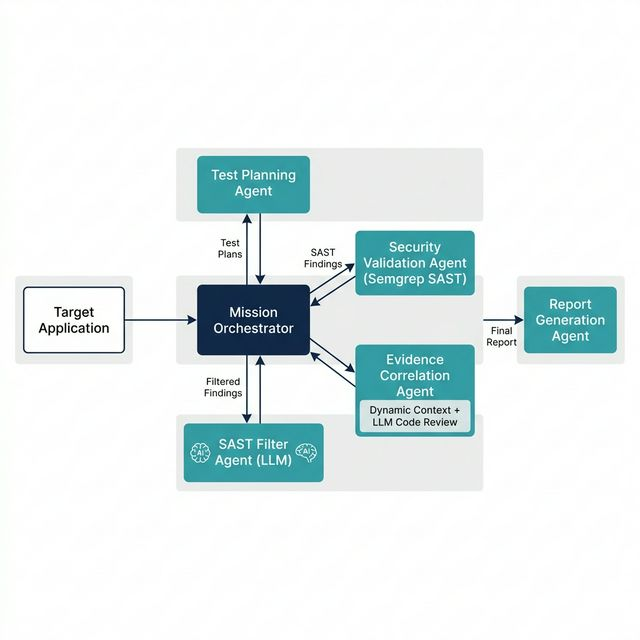
\includegraphics[width=\columnwidth]{fig_architecture.png}
  \caption{QASecClaw system architecture. The Mission Orchestrator coordinates specialized agents through sequential mission phases: Test Planning, Security Validation (Semgrep SAST), Evidence Correlation with LLM-based SAST filtering, and Report Generation.}
  \label{fig:architecture}
\end{figure}

\subsection{Mission Orchestrator}
The Mission Orchestrator implements a finite state machine that manages the analysis lifecycle through the following phases:

\begin{enumerate}
    \item \textbf{Initialization}: Configures the target application, resolves source paths, and creates a unique run identifier for audit trails.
    \item \textbf{Test Planning}: Delegates to the Test Planning Agent to generate coverage and vulnerability testing plans based on the target's file structure and API specification.
    \item \textbf{Active Testing}: Coordinates UI and API testing agents for dynamic analysis (when applicable).
    \item \textbf{Security Validation}: Invokes the Security Validation Agent, which executes Semgrep SAST against the target source code.
    \item \textbf{Evidence Correlation}: The core value proposition — correlates findings across all agents and invokes the SAST Filter Agent to reduce false positives.
    \item \textbf{Report Generation}: Synthesizes a comprehensive security assessment report.
\end{enumerate}

\subsection{Security Validation Agent}
The Security Validation Agent wraps Semgrep~\cite{semgrep2023}, executing it against the target source code with the \texttt{auto} ruleset configuration. It parses Semgrep's JSON output to extract structured \texttt{SecurityFinding} objects containing the check ID (used as \texttt{vulnerabilityType}), file location, severity, and description. This normalization enables downstream agents to process findings uniformly regardless of the underlying SAST engine.

\subsection{SAST Filter Agent}
\label{sec:sast-filter}
The SAST Filter Agent is the architectural innovation central to QASecClaw's false positive reduction capability. When invoked during the Evidence Correlation phase, it processes SAST findings that lack dynamic execution context (i.e., findings that could not be correlated with UI traces, API logs, or runtime behavior).

For each batch of uncorrelated findings, the agent:
\begin{enumerate}
    \item \textbf{Extracts source code}: Reads the full source file associated with each finding.
    \item \textbf{Constructs a context-aware prompt}: Includes the reported vulnerability type, CWE identifier, file location, and complete source code for each finding in the batch.
    \item \textbf{Queries the LLM}: Submits the prompt to a code-specialized LLM (Qwen 3.5 Plus) with instructions to analyze data flows from input sources to execution sinks and classify each finding as a true positive or false positive.
    \item \textbf{Applies fail-open safety}: If the LLM fails to respond or returns malformed output for a batch, all findings in that batch are retained to prevent inadvertent suppression of real vulnerabilities.
\end{enumerate}

The system prompt instructs the LLM to perform vulnerability-type-specific analysis:
\begin{itemize}
    \item For injection vulnerabilities (SQLi, Command Injection, XSS, LDAP Injection, XPath Injection): trace user input to execution sinks and verify absence of sanitization/parameterization.
    \item For path traversal: verify file I/O operations use canonicalized paths with proper validation.
    \item For cryptographic vulnerabilities: identify use of weak algorithms or insecure configurations.
\end{itemize}

Findings are processed in batches of 15 to balance API throughput against context window limitations.

\subsection{Evidence Correlation Agent}
The Evidence Correlation Agent implements a two-pass filtering strategy:
\begin{enumerate}
    \item \textbf{Dynamic correlation} (Pass 1): Links SAST findings with evidence from UI traces, API logs, and system anomalies. Findings with dynamic execution evidence are immediately classified as verified.
    \item \textbf{LLM code review} (Pass 2): Remaining uncorrelated findings are forwarded to the SAST Filter Agent for deep code analysis.
\end{enumerate}

This dual-pass approach ensures that QASecClaw can operate effectively both in scenarios with rich dynamic context (live applications) and in purely static analysis scenarios (code benchmarks).

% ═══════════════════════════════════════════════════════════════════════════
%  IV. EXPERIMENTAL SETUP
% ═══════════════════════════════════════════════════════════════════════════
\section{Experimental Setup}
\label{sec:setup}

\subsection{Research Questions}
We investigate the following research questions:

\begin{itemize}
    \item \textbf{RQ1}: How does QASecClaw compare to standalone SAST tools on standardized vulnerability benchmarks in terms of Precision, Recall, and F1-Score?
    \item \textbf{RQ2}: To what extent does QASecClaw's LLM-augmented filtering reduce false positives compared to individual SAST scanners?
    \item \textbf{RQ3}: How does detection performance vary across CWE categories?
\end{itemize}

\subsection{Dataset: OWASP Benchmark v1.2}
The \textbf{OWASP Benchmark Project}~\cite{owasp2023benchmark} is a free and open test suite designed to evaluate the accuracy, coverage, and speed of automated software vulnerability detection tools. Version 1.2 comprises \textbf{2,740 Java test cases}, each designed as a self-contained servlet that either contains a real, exploitable vulnerability (a true positive) or is intentionally designed to mimic a vulnerability pattern without being exploitable (a false positive intended to trick scanners).

Each test case is identified by a filename of the form \texttt{BenchmarkTestNNNNN.java}, and the ground truth is provided in \texttt{expectedresults-1.2.csv}, which maps each test case to its CWE category and a boolean label indicating whether the test case represents a real vulnerability.

\begin{table}[t]
\centering
\caption{OWASP Benchmark v1.2 Dataset Distribution}
\label{tab:dataset}
\begin{tabular}{llrrr}
\toprule
\textbf{CWE} & \textbf{Category} & \textbf{Vuln.} & \textbf{Safe} & \textbf{Total} \\
\midrule
CWE-22  & Path Traversal           & 133  & 135  & 268 \\
CWE-78  & Command Injection        & 126  & 125  & 251 \\
CWE-79  & Cross-Site Scripting     & 246  & 209  & 455 \\
CWE-89  & SQL Injection            & 272  & 232  & 504 \\
CWE-90  & LDAP Injection           & 27   & 32   & 59  \\
CWE-327 & Weak Cryptography        & 130  & 116  & 246 \\
CWE-328 & Weak Hashing             & 129  & 107  & 236 \\
CWE-330 & Weak Randomness          & 218  & 275  & 493 \\
CWE-501 & Trust Boundary Violation & 83   & 43   & 126 \\
CWE-614 & Insecure Cookie          & 36   & 31   & 67  \\
CWE-643 & XPath Injection          & 15   & 20   & 35  \\
\midrule
\multicolumn{2}{l}{\textbf{Total}} & \textbf{1,415} & \textbf{1,325} & \textbf{2,740} \\
\bottomrule
\end{tabular}
\end{table}

\subsection{Baseline}
We use \textbf{Semgrep Community Edition}~\cite{semgrep2023} as the SAST baseline, configured with the \texttt{auto} ruleset (which includes the \texttt{p/default} and community rulesets). Semgrep was selected because: (1) it is a widely-adopted open-source SAST tool, (2) it supports Java analysis, and (3) it produces structured JSON output amenable to automated evaluation.

\subsection{Evaluation Metrics}
We adopt standard information retrieval metrics used in the security tool evaluation literature~\cite{delaitre2015nist}:
\begin{align}
    \text{Precision} &= \frac{TP}{TP + FP} \label{eq:precision} \\
    \text{Recall (TPR)} &= \frac{TP}{TP + FN} \label{eq:recall} \\
    \text{F1-Score} &= 2 \times \frac{\text{Precision} \times \text{Recall}}{\text{Precision} + \text{Recall}} \label{eq:f1} \\
    \text{FPR} &= \frac{FP}{FP + TN} \label{eq:fpr} \\
    \text{Youden's \textit{J}} &= \text{TPR} - \text{FPR} \label{eq:youden}
\end{align}

Youden's J statistic~\cite{youden1950index} is the OWASP Benchmark Project's primary ranking metric, as it captures both detection and false alarm rates in a single value.

\subsection{Experimental Procedure}
The evaluation was conducted in a two-stage pipeline:
\begin{enumerate}
    \item \textbf{Baseline assessment}: Standalone Semgrep was executed against the full OWASP Benchmark test code directory. The JSON output was parsed and normalized to extract unique test case findings.
    \item \textbf{QASecClaw assessment}: The complete QASecClaw pipeline was executed, including Semgrep scanning followed by the SAST Filter Agent's LLM-based code review for all uncorrelated findings.
\end{enumerate}

Both tools' findings were cross-referenced against the OWASP ground truth at the file level (\texttt{BenchmarkTestNNNNN}) to compute confusion matrix entries and derived metrics.

\subsection{Implementation Details}
QASecClaw is implemented in TypeScript running on Node.js. The SAST Filter Agent uses the \textbf{Qwen 3.5 Plus} model via API for code review. Findings are processed in batches of 15 files to manage API throughput and context limitations. The complete pipeline execution (including Semgrep scanning, LLM-based filtering, and scoring) completed in approximately \textbf{45 minutes} on a standard development workstation.

% ═══════════════════════════════════════════════════════════════════════════
%  V. RESULTS
% ═══════════════════════════════════════════════════════════════════════════
\section{Results}
\label{sec:results}

\subsection{RQ1: Overall Performance Comparison}

Table~\ref{tab:overall} presents the aggregate performance metrics for QASecClaw and the Semgrep baseline on the complete OWASP Benchmark v1.2. Fig.~\ref{fig:overall} provides a visual comparison.

\begin{table}[t]
\centering
\caption{Overall Performance on OWASP Benchmark v1.2 (2,740 test cases)}
\label{tab:overall}
\begin{tabular}{lccccc}
\toprule
\textbf{Tool} & \textbf{Prec.} & \textbf{Recall} & \textbf{F1} & \textbf{FPR} & \textbf{$J$} \\
\midrule
QASecClaw & \textbf{0.951} & 0.871  & \textbf{0.909} & \textbf{0.048} & \textbf{0.823} \\
Semgrep   & 0.695          & \textbf{0.900} & 0.784          & 0.423          & 0.477 \\
\bottomrule
\end{tabular}
\end{table}

\begin{figure}[t]
  \centering
  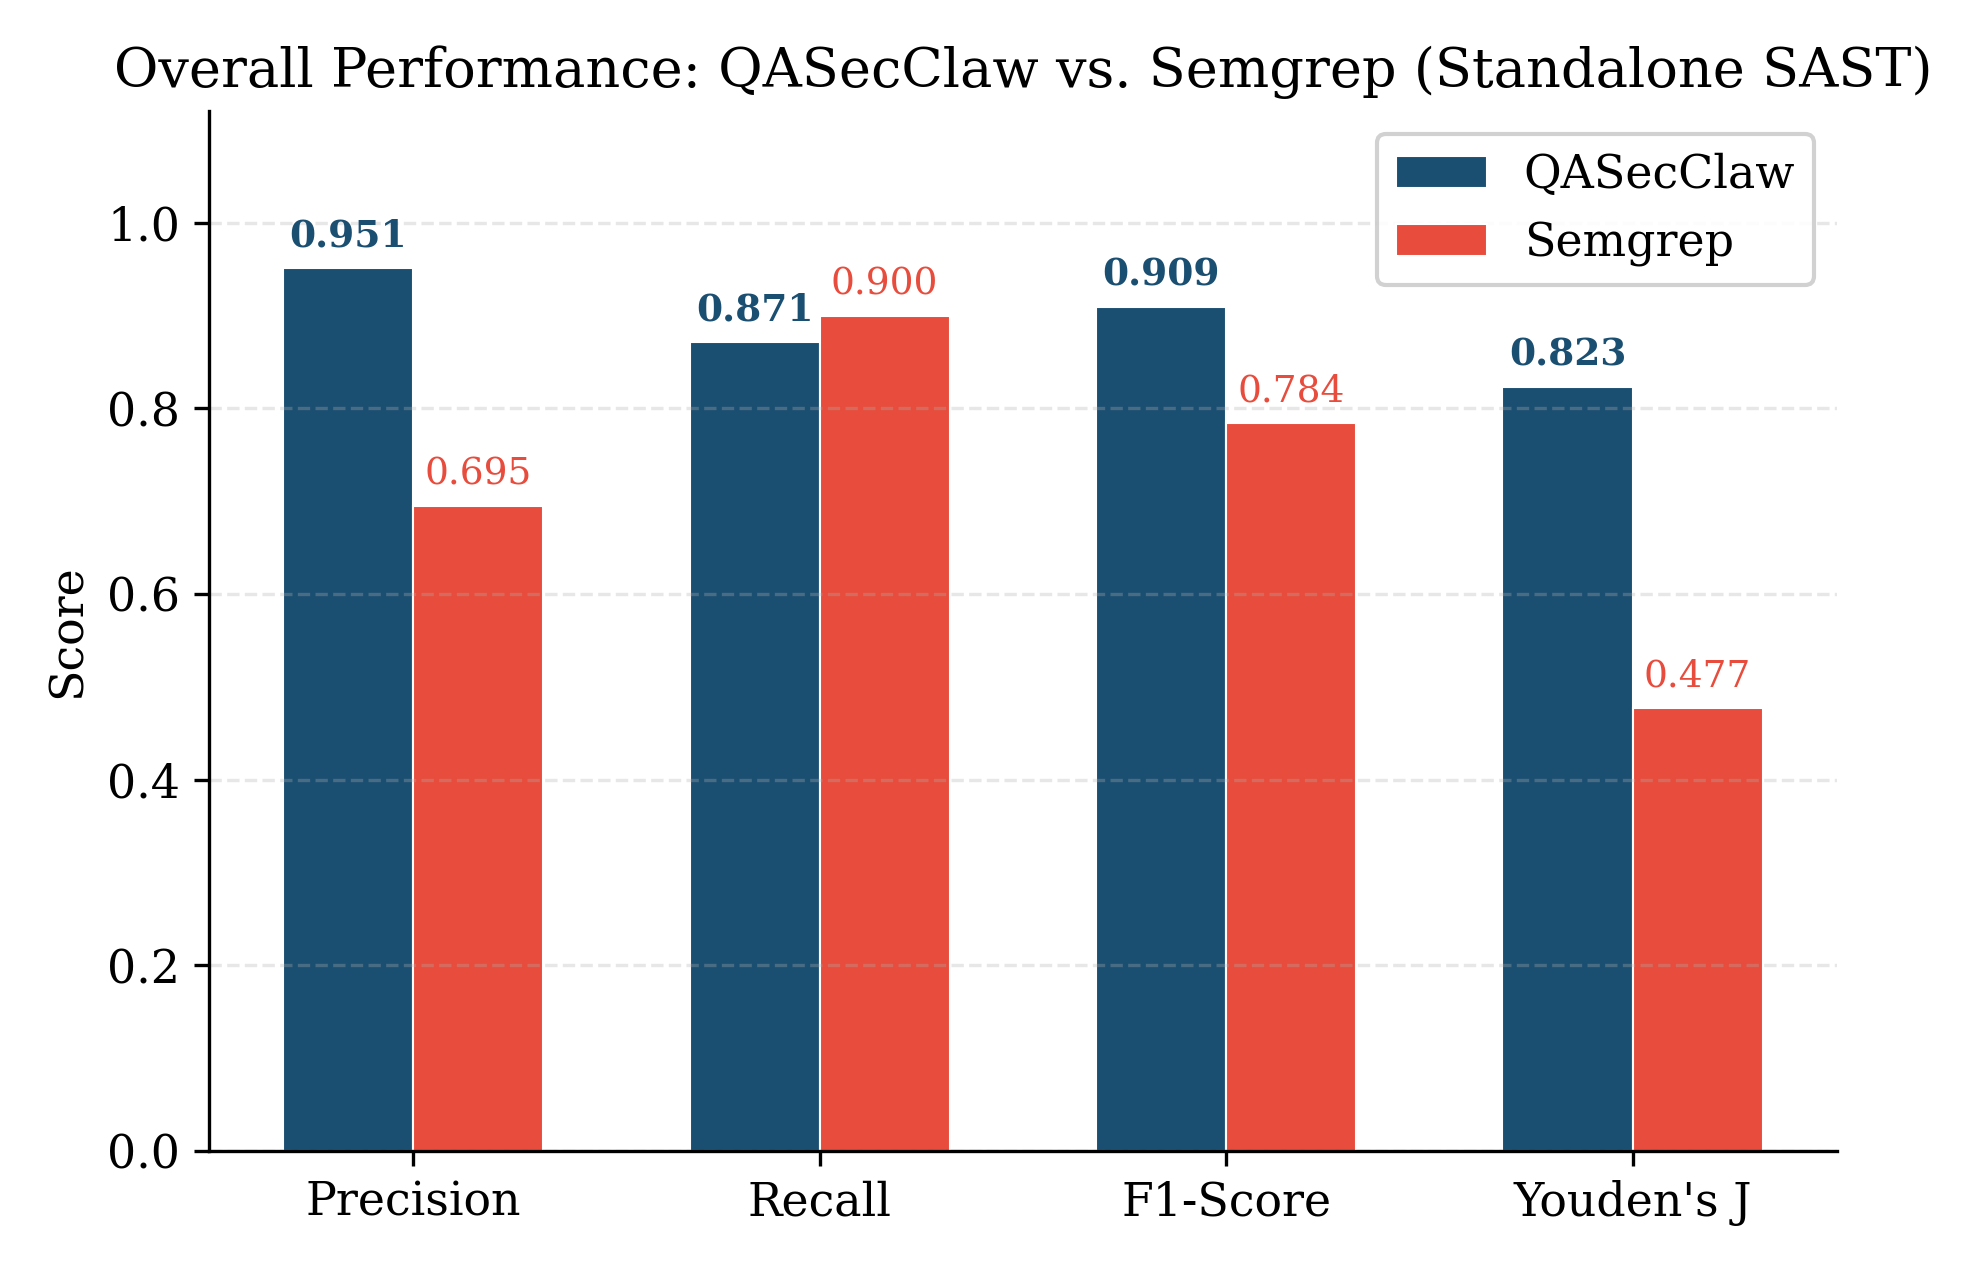
\includegraphics[width=\columnwidth]{fig_overall_comparison.png}
  \caption{Aggregate metric comparison between QASecClaw and standalone Semgrep across the OWASP Benchmark v1.2 dataset.}
  \label{fig:overall}
\end{figure}

QASecClaw achieves an F1-score of \textbf{0.909}, representing a \textbf{16.0\%} improvement over Semgrep's 0.784. The improvement is predominantly driven by a dramatic increase in Precision from 0.695 to 0.951, while Recall experiences a modest decrease from 0.900 to 0.871 (a 3.2\% relative reduction). The False Positive Rate drops from 0.423 to 0.048 — a reduction of \textbf{88.6\%}. Correspondingly, Youden's J increases from 0.477 to 0.823, indicating substantially better discriminative ability.

\textbf{Answer to RQ1}: QASecClaw significantly outperforms standalone Semgrep on the OWASP Benchmark, achieving a 16.0\% higher F1-score through dramatic false positive reduction with minimal recall loss.

\subsection{RQ2: False Positive Reduction Analysis}

\begin{table}[t]
\centering
\caption{Confusion Matrix Comparison}
\label{tab:confusion}
\begin{tabular}{lrrrr}
\toprule
\textbf{Tool} & \textbf{TP} & \textbf{FP} & \textbf{TN} & \textbf{FN} \\
\midrule
QASecClaw & 1,233 & \textbf{64}  & \textbf{1,261} & 182 \\
Semgrep   & 1,273 & 560          & 765            & 142 \\
\midrule
\textbf{$\Delta$} & $-$40 & $-$496 & +496 & +40 \\
\bottomrule
\end{tabular}
\end{table}

Table~\ref{tab:confusion} presents the confusion matrix comparison. QASecClaw correctly reclassified \textbf{496 false positives} as true negatives, while only misclassifying 40 true positives as false negatives. This yields a false positive suppression ratio of 88.6\% ($496/560$) with a true positive loss ratio of only 3.1\% ($40/1273$).

Fig.~\ref{fig:fp_reduction} illustrates the per-CWE false positive reduction, showing consistent improvements across all vulnerability categories that exhibited false positives in the baseline.

\begin{figure}[t]
  \centering
  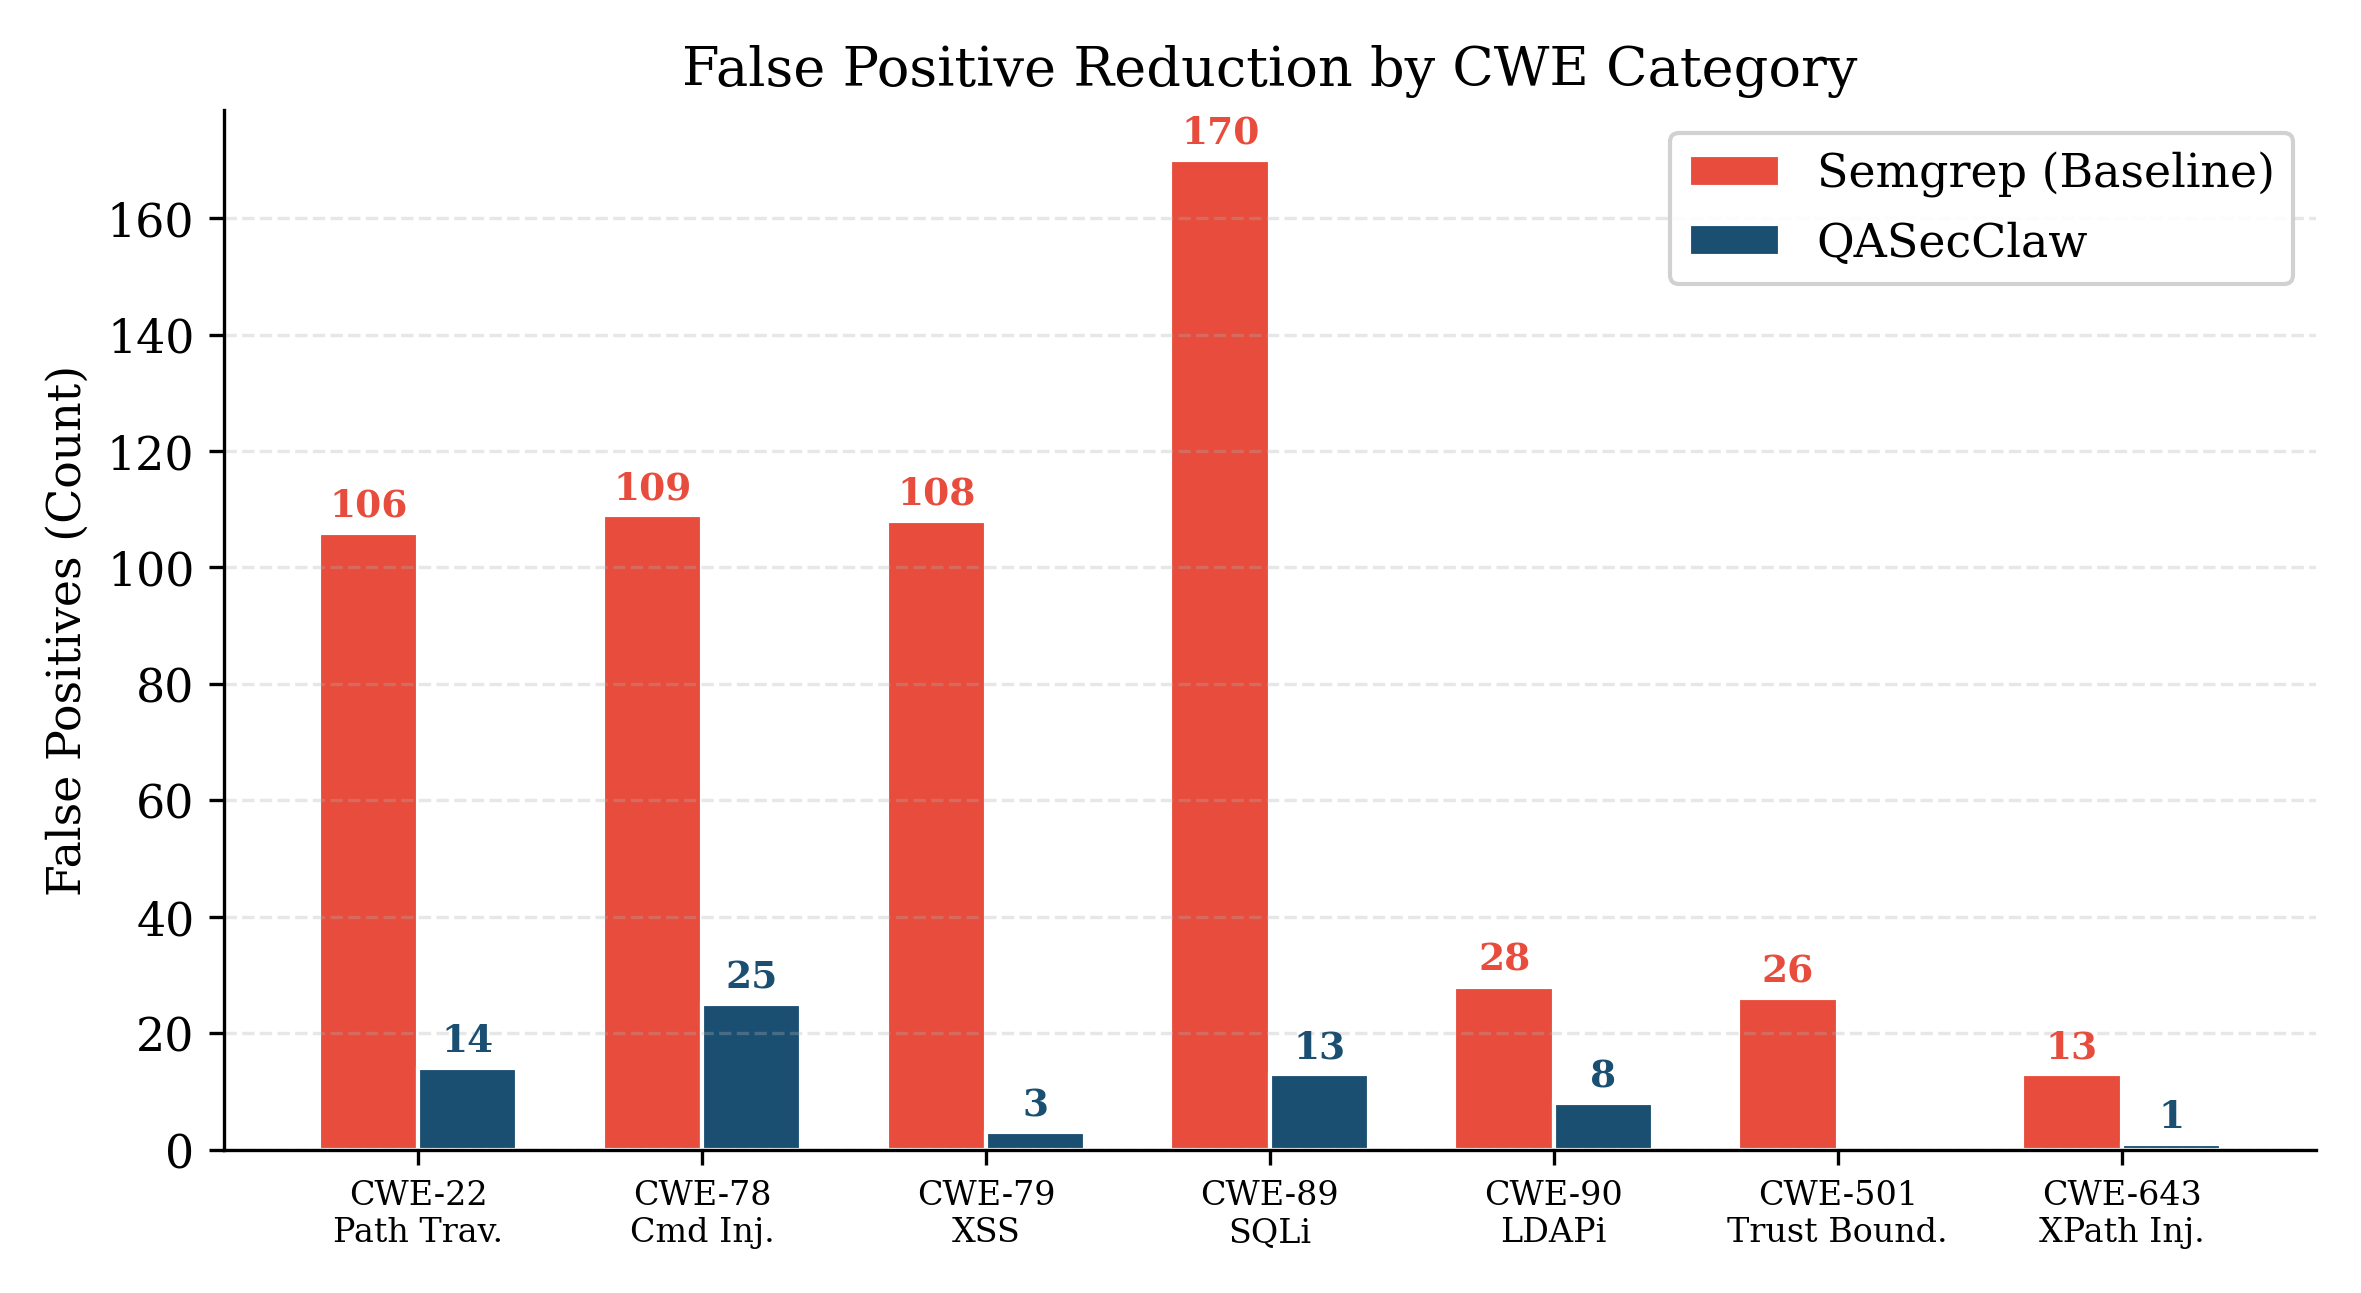
\includegraphics[width=\columnwidth]{fig_fp_reduction.png}
  \caption{Per-CWE false positive counts for Semgrep vs.\ QASecClaw. QASecClaw reduces false positives across all affected CWE categories.}
  \label{fig:fp_reduction}
\end{figure}

\textbf{Answer to RQ2}: QASecClaw's LLM-augmented filtering eliminates 88.6\% of false positives produced by standalone SAST, with a favorable trade-off of only 3.1\% recall loss.

\subsection{RQ3: Per-CWE Performance Analysis}

Table~\ref{tab:per_cwe} presents the detailed per-CWE breakdown. Fig.~\ref{fig:per_cwe_f1} and Fig.~\ref{fig:pr_scatter} provide visual comparisons.

\begin{table*}[t]
\centering
\caption{Per-CWE Performance Breakdown: QASecClaw vs.\ Semgrep}
\label{tab:per_cwe}
\begin{tabular}{ll|ccc|ccc|cc}
\toprule
& & \multicolumn{3}{c|}{\textbf{QASecClaw}} & \multicolumn{3}{c|}{\textbf{Semgrep}} & \multicolumn{2}{c}{\textbf{$\Delta$ F1}} \\
\textbf{CWE} & \textbf{Category} & \textbf{Prec.} & \textbf{Rec.} & \textbf{F1} & \textbf{Prec.} & \textbf{Rec.} & \textbf{F1} & \textbf{Abs.} & \textbf{Rel.} \\
\midrule
CWE-22  & Path Traversal       & 0.895 & 0.895 & 0.895 & 0.531 & 0.902 & 0.669 & +0.226 & +33.8\% \\
CWE-78  & Command Injection    & 0.821 & 0.913 & 0.865 & 0.518 & 0.929 & 0.665 & +0.200 & +30.1\% \\
CWE-79  & XSS                  & 0.985 & 0.821 & 0.896 & 0.652 & 0.821 & 0.727 & +0.169 & +23.3\% \\
CWE-89  & SQL Injection        & 0.951 & 0.930 & 0.941 & 0.598 & 0.930 & 0.728 & +0.213 & +29.2\% \\
CWE-90  & LDAP Injection       & 0.765 & 0.963 & 0.853 & 0.482 & 0.963 & 0.642 & +0.211 & +32.9\% \\
CWE-327 & Weak Cryptography    & 1.000 & 0.992 & 0.996 & 1.000 & 1.000 & 1.000 & $-$0.004 & $-$0.4\% \\
CWE-328 & Weak Hashing         & 1.000 & 0.667 & 0.800 & 1.000 & 0.690 & 0.817 & $-$0.017 & $-$2.0\% \\
CWE-330 & Weak Randomness      & 1.000 & 1.000 & 1.000 & 1.000 & 1.000 & 1.000 & 0.000 & 0.0\% \\
CWE-501 & Trust Bound.\ Viol.  & 1.000 & 0.422 & 0.593 & 0.723 & 0.819 & 0.768 & $-$0.175 & $-$22.8\% \\
CWE-614 & Insecure Cookie      & 1.000 & 1.000 & 1.000 & 1.000 & 1.000 & 1.000 & 0.000 & 0.0\% \\
CWE-643 & XPath Injection      & 0.933 & 0.933 & 0.933 & 0.519 & 0.933 & 0.667 & +0.266 & +39.9\% \\
\bottomrule
\end{tabular}
\end{table*}

\begin{figure}[t]
  \centering
  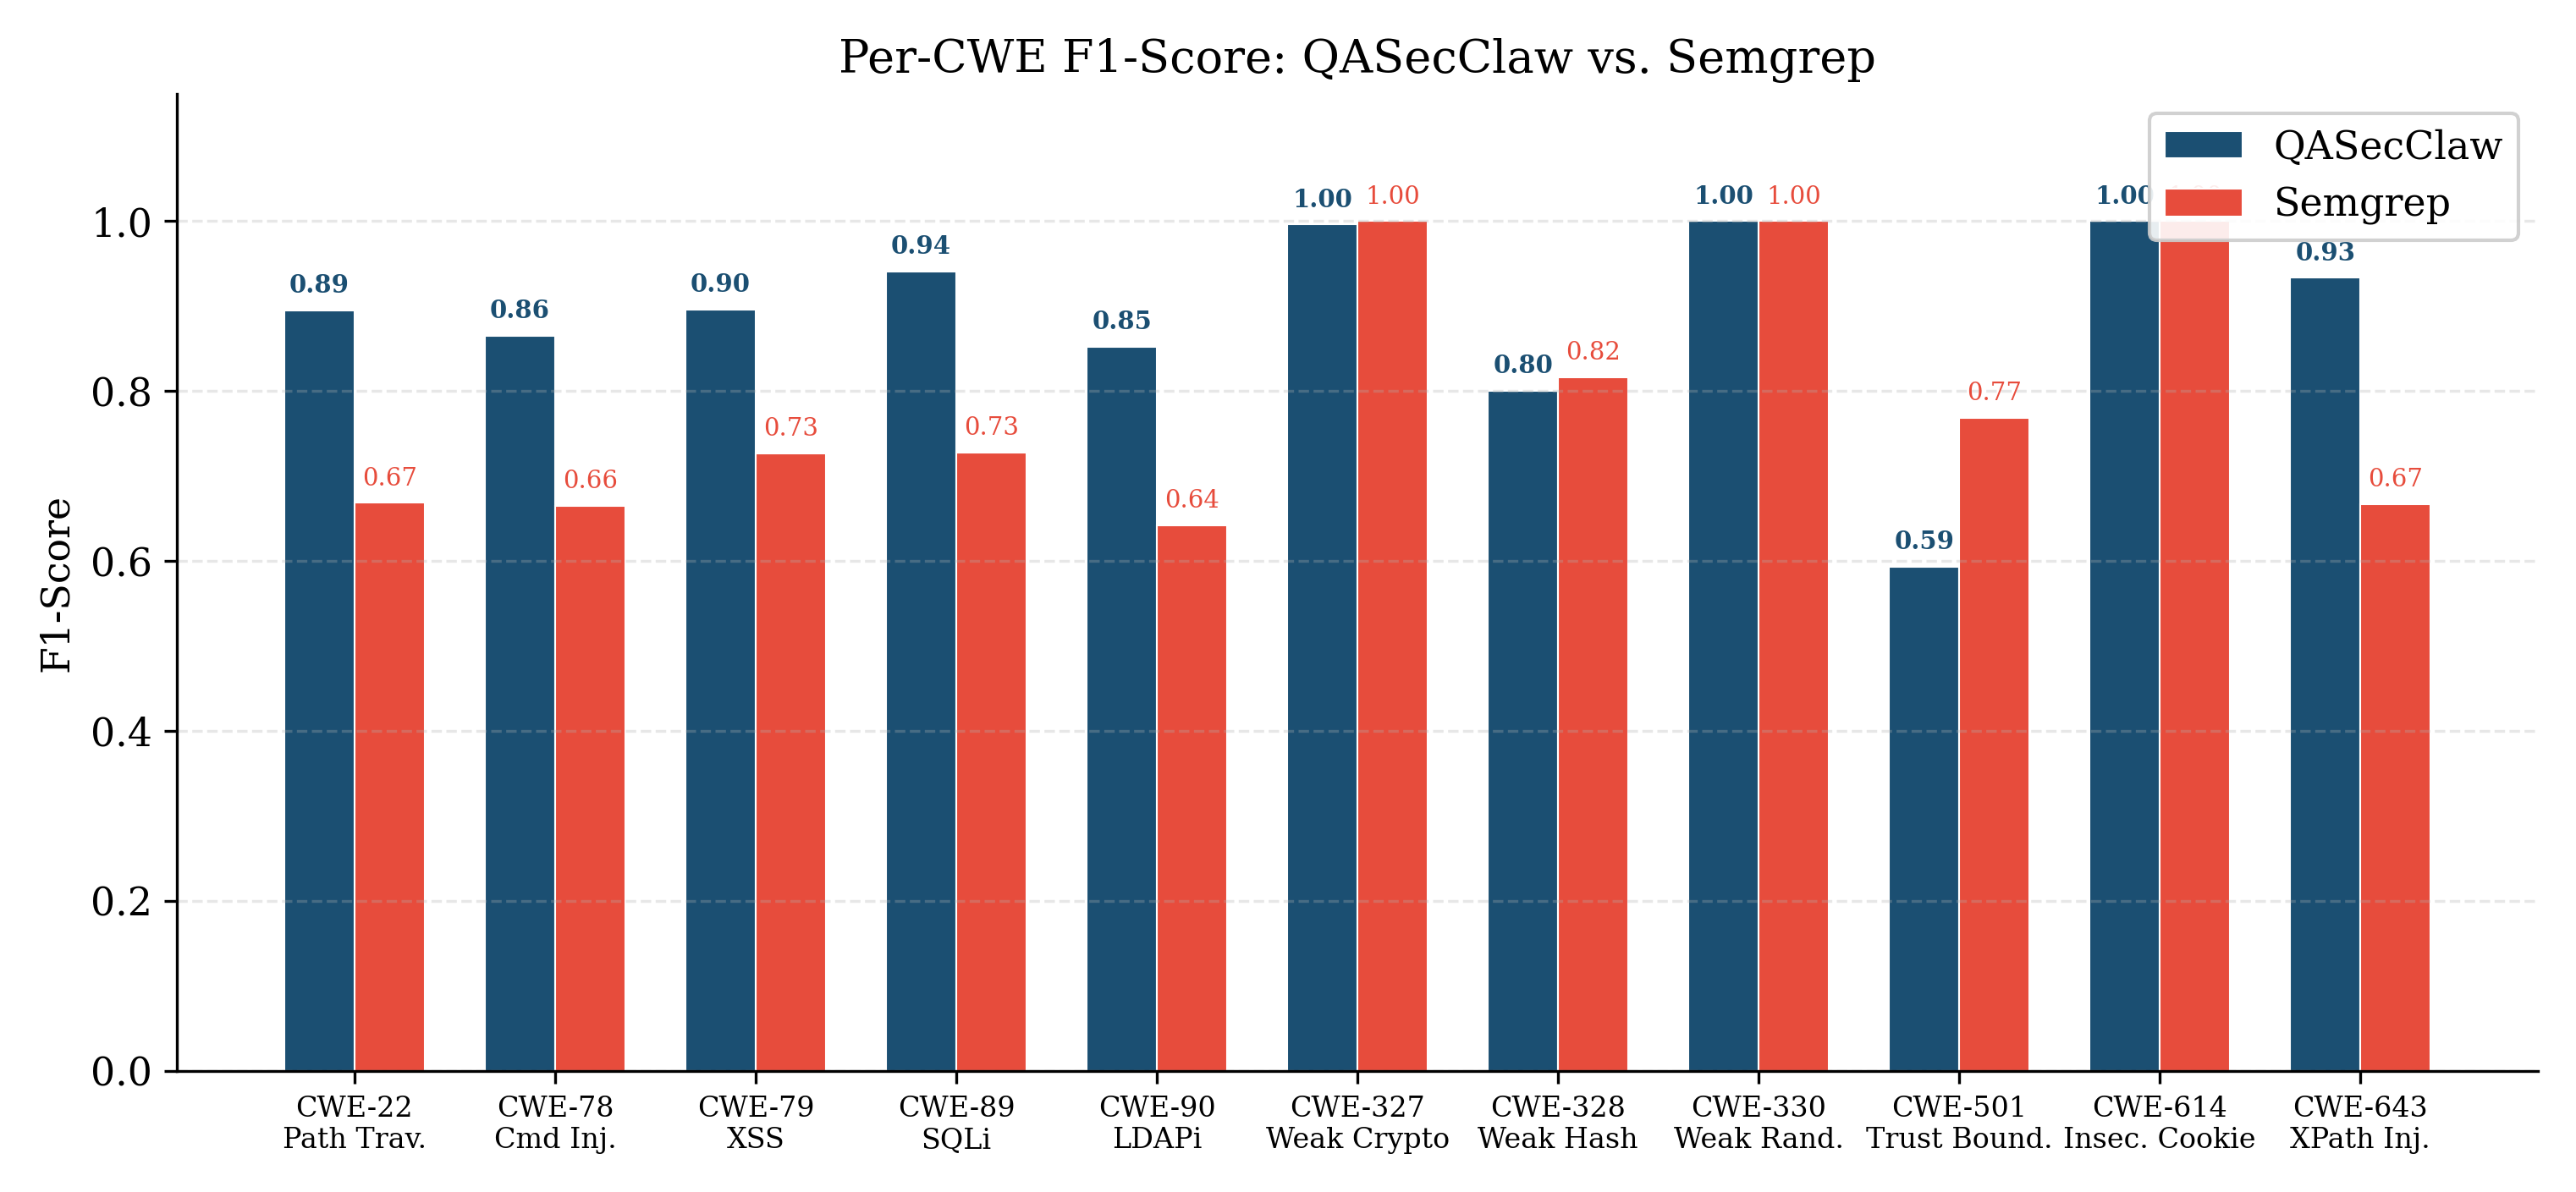
\includegraphics[width=\columnwidth]{fig_per_cwe_f1.png}
  \caption{Per-CWE F1-score comparison. QASecClaw achieves substantial F1 improvements on injection-class CWEs while maintaining parity on cryptographic CWEs.}
  \label{fig:per_cwe_f1}
\end{figure}

\begin{figure}[t]
  \centering
  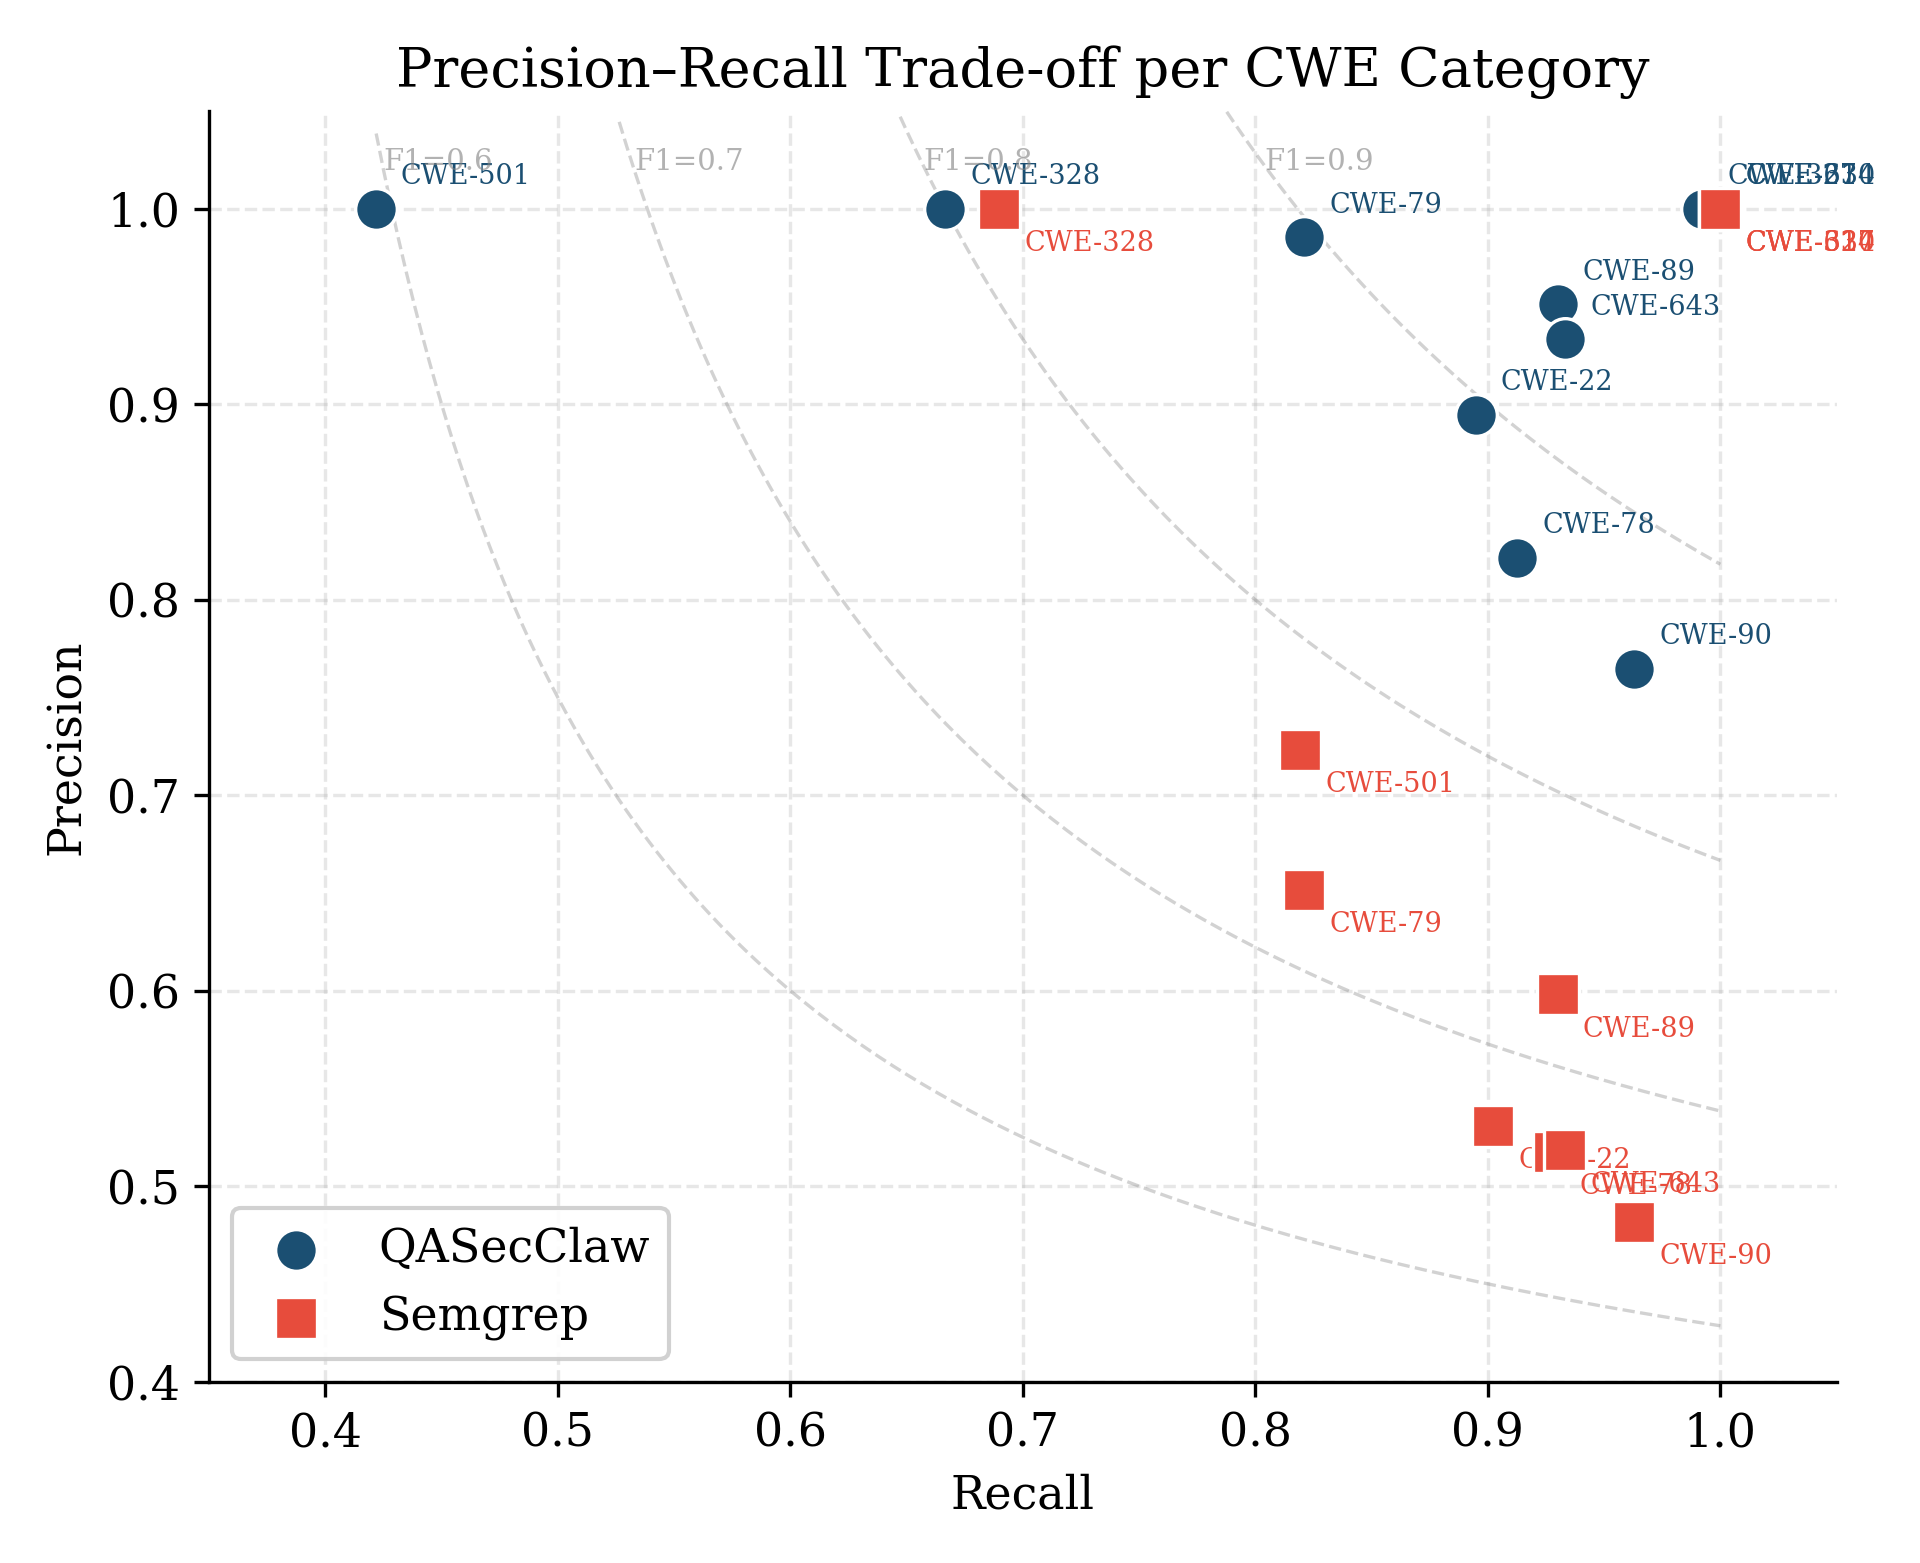
\includegraphics[width=\columnwidth]{fig_precision_recall.png}
  \caption{Precision--Recall scatter plot per CWE category. QASecClaw points cluster in the high-precision, high-recall region (upper right), while Semgrep points exhibit high recall but low precision for injection CWEs.}
  \label{fig:pr_scatter}
\end{figure}

\textbf{Injection vulnerabilities} (CWE-22, 78, 79, 89, 90, 643) show the largest improvements, with F1-score gains ranging from +0.169 (XSS) to +0.266 (XPath Injection). These CWEs are historically problematic for SAST tools because the distinction between exploitable and safe code depends on subtle data flow analysis that pattern-matching rules struggle to capture.

\textbf{Cryptographic vulnerabilities} (CWE-327, 328, 330) maintain near-parity with the baseline. This is expected because Semgrep's rules for these categories already achieve near-perfect precision (both tools report 0 false positives), meaning there are no false positives for the LLM filter to correct.

\textbf{CWE-501 (Trust Boundary Violation)} is the only category where QASecClaw's F1-score is notably lower than the baseline ($-$22.8\%). Investigation reveals that the LLM filter was overly conservative for this category, correctly eliminating all 26 false positives from Semgrep but also misclassifying 48 true positives as benign. This suggests that trust boundary violations require more specialized prompting strategies.

\textbf{Answer to RQ3}: QASecClaw delivers the largest improvements on injection-class CWEs (F1 gains of +17\% to +40\%), maintains parity on well-detected cryptographic CWEs, and shows room for improvement on trust boundary violations.

% ═══════════════════════════════════════════════════════════════════════════
%  VI. DISCUSSION
% ═══════════════════════════════════════════════════════════════════════════
\section{Discussion}
\label{sec:discussion}

\subsection{Practical Implications}
The 88.6\% reduction in false positives has significant practical implications for software development teams. In a typical CI/CD pipeline, reducing the number of findings that require manual triage from 560 to 64 can save substantial developer hours per scan cycle. Moreover, the high precision (0.951) means that when QASecClaw flags a finding, developers can have high confidence that it represents a real vulnerability, improving developer trust in the tooling.

\subsection{Cost-Accuracy Trade-off}
Using an LLM for code review introduces API costs proportional to the number of findings processed. In our evaluation, approximately 1,833 unique test configurations were processed through the LLM in batches of 15, requiring approximately 122 API calls. The total execution time was approximately 45 minutes, with the majority spent on LLM inference. For organizations processing large codebases, this cost must be weighed against the savings from reduced manual triage.

\subsection{Fail-Open Safety Design}
A critical design decision in QASecClaw is the fail-open policy: when the LLM fails to return a valid classification for a batch (due to API errors, rate limits, or malformed responses), all findings in that batch are retained. This ensures that transient LLM failures cannot cause real vulnerabilities to be silently suppressed. In our evaluation, approximately 10--15 batches experienced failures (primarily due to network interruptions), and their findings were correctly retained.

% ═══════════════════════════════════════════════════════════════════════════
%  VII. THREATS TO VALIDITY
% ═══════════════════════════════════════════════════════════════════════════
\section{Threats to Validity}
\label{sec:threats}

\subsection{Internal Validity}
\textbf{LLM non-determinism}: LLM responses may vary between runs due to sampling parameters. We mitigate this by using structured JSON output parsing and the fail-open safety mechanism. Future work should include multiple runs to quantify variance.

\textbf{Batch failures}: Network interruptions during the evaluation caused approximately 10--15 batch failures. The fail-open design retained these findings, potentially inflating the false positive count slightly.

\subsection{External Validity}
\textbf{Synthetic benchmark}: The OWASP Benchmark consists of synthetic test cases that may not fully represent the complexity and diversity of real-world vulnerable code. However, it remains the industry standard for SAST tool evaluation and provides controlled, reproducible ground truth.

\textbf{Language and framework scope}: Our evaluation is limited to Java web applications. Generalization to other languages and frameworks requires additional evaluation.

\textbf{Single SAST baseline}: We evaluate against Semgrep only. Comparison with additional SAST tools (e.g., SonarQube, Fortify, Checkmarx) would strengthen the findings.

\subsection{Construct Validity}
\textbf{File-level matching}: Our scoring matches findings at the file level (\texttt{BenchmarkTestNNNNN}), not at the specific vulnerability instance level. This could slightly affect metrics if a tool reports a finding in the correct file but for the wrong vulnerability pattern.

% ═══════════════════════════════════════════════════════════════════════════
%  VIII. CONCLUSION
% ═══════════════════════════════════════════════════════════════════════════
\section{Conclusion and Future Work}
\label{sec:conclusion}

We presented QASecClaw, a multi-agent framework that augments static application security testing with LLM-driven contextual code review. Our evaluation on the complete OWASP Benchmark v1.2 (2,740 test cases across 11 CWE categories) demonstrates that QASecClaw achieves an F1-score of 0.909, outperforming standalone Semgrep (F1: 0.784) by reducing false positives by 88.6\% with only a 3.1\% loss in recall. These results validate the viability of LLM-augmented multi-agent architectures as a practical approach to improving the signal-to-noise ratio of SAST tools.

\textbf{Future work} includes: (1) extending the evaluation to real-world open-source projects with known CVEs, (2) incorporating additional SAST engines and dynamic analysis tools, (3) optimizing the SAST Filter Agent's prompting strategies for under-performing CWE categories (notably CWE-501), (4) evaluating the framework across multiple LLM providers to assess model sensitivity, and (5) investigating the cost-effectiveness trade-off at enterprise scale.

% ═══════════════════════════════════════════════════════════════════════════
%  REFERENCES
% ═══════════════════════════════════════════════════════════════════════════
\bibliographystyle{IEEEtran}

\begin{thebibliography}{99}

\bibitem{chess2004static}
B.~Chess and J.~West, \textit{Secure Programming with Static Analysis}. Addison-Wesley, 2007.

\bibitem{johnson2013don}
B.~Johnson, Y.~Song, E.~Murphy-Hill, and R.~Bowdidge, ``Why don't software developers use static analysis tools to find bugs?'' in \textit{Proc.\ ICSE}, 2013, pp.~672--681.

\bibitem{sadowski2015tricorder}
C.~Sadowski, J.~van Gogh, C.~Jaspan, E.~Söderberg, and C.~Winter, ``Tricorder: Building a program analysis ecosystem,'' in \textit{Proc.\ ICSE}, 2015, pp.~598--608.

\bibitem{chen2021evaluating}
M.~Chen, J.~Tworek, H.~Jun, Q.~Yuan, et~al., ``Evaluating large language models trained on code,'' arXiv:2107.03374, 2021.

\bibitem{feng2020codebert}
Z.~Feng, D.~Guo, D.~Tang, et~al., ``CodeBERT: A pre-trained model for programming and natural languages,'' in \textit{Proc.\ EMNLP Findings}, 2020, pp.~1536--1547.

\bibitem{wooldridge2009introduction}
M.~Wooldridge, \textit{An Introduction to MultiAgent Systems}. Wiley, 2009.

\bibitem{semgrep2023}
Semgrep, ``Semgrep: Lightweight static analysis for many languages,'' 2023. [Online]. Available: \url{https://semgrep.dev}

\bibitem{sonarqube2023}
SonarSource, ``SonarQube,'' 2023. [Online]. Available: \url{https://www.sonarsource.com/products/sonarqube/}

\bibitem{lam2017combining}
P.~Lam, E.~Bodden, O.~Lhoták, and L.~Hendren, ``The Soot framework for Java program analysis: A retrospective,'' in \textit{Cetus Users and Compiler Infrastructure Workshop}, 2011.

\bibitem{delaitre2015nist}
A.~Delaitre, B.~Stivalet, E.~Fong, and V.~Okun, ``Evaluating bug finders --- Test and measurement of static code analyzers,'' in \textit{Proc.\ IEEE ICSME Workshop}, 2015.

\bibitem{flynn2018prioritizing}
L.~Flynn, W.~Snavely, D.~Svoboda, et~al., ``Prioritizing alerts from multiple static analysis tools, using classification models,'' in \textit{Proc.\ IEEE/ACM International Workshop on Software Engineering for Smart Cyber-Physical Systems}, 2018.

\bibitem{li2021vulnerability}
Z.~Li, D.~Zou, S.~Xu, et~al., ``VulDeePecker: A deep learning-based system for vulnerability detection,'' in \textit{Proc.\ NDSS}, 2018.

\bibitem{zhou2019devign}
Y.~Zhou, S.~Liu, J.~Siow, X.~Du, and Y.~Liu, ``Devign: Effective vulnerability identification by learning comprehensive program semantics via graph neural networks,'' in \textit{Proc.\ NeurIPS}, 2019.

\bibitem{thapa2022transformer}
C.~Thapa, S.~I.~Jang, M.~E.~Ahmed, et~al., ``Transformer-based language models for software vulnerability detection,'' in \textit{Proc.\ ACSAC}, 2022.

\bibitem{pearce2023examining}
H.~Pearce, B.~Ahmad, B.~Tan, et~al., ``Examining zero-shot vulnerability repair with large language models,'' in \textit{Proc.\ IEEE S\&P}, 2023.

\bibitem{li2023large}
H.~Li, Y.~Hao, Y.~Zhai, and Z.~Qian, ``The hitchhiker's guide to program analysis: A journey with large language models,'' arXiv:2308.00245, 2023.

\bibitem{hong2023metagpt}
S.~Hong, X.~Zhuge, J.~Chen, et~al., ``MetaGPT: Meta programming for a multi-agent collaborative framework,'' arXiv:2308.00352, 2023.

\bibitem{qian2023chatdev}
C.~Qian, X.~Cong, C.~Yang, et~al., ``Communicative agents for software development,'' arXiv:2307.07924, 2023.

\bibitem{owasp2023benchmark}
OWASP Foundation, ``OWASP Benchmark Project,'' 2023. [Online]. Available: \url{https://owasp.org/www-project-benchmark/}

\bibitem{youden1950index}
W.~J.~Youden, ``Index for rating diagnostic tests,'' \textit{Cancer}, vol.~3, no.~1, pp.~32--35, 1950.

\end{thebibliography}

\end{document}
